\def\agileboxref{\href{https://goo.gl/mmWyZF}{Agile Project Management Box
      Set. Agile Project Management QuickStart and Mastery
      Guides. ClydeBank Media}.}

\lecture{Abordagens Ágeis}{agile}
\lecturetitle{\insertlecture}{\course}

\frame{\maketitle}

\section{\insertlecture}

\begin{frame}{Referências}

  \begin{itemize}
  \item Ian
    Sommerville. \href{https://feituverava.bv3.digitalpages.com.br/users/publications/9788579361081/pages/39}{Engenharia
      de Software, Capítulo~3, página~38}. Pearson, 9$^a$ edição, 2011.
  \item \agileboxref
  \end{itemize}
\end{frame}

\begin{frame}{Manifesto Ágil}
  \begin{itemize}[<+-| alert@+>]\setbeamercovered{transparent}
  \item No início de 2001, 17 desenvolvedores lançaram um
    \href{http://agilemanifesto.org/}{Manifesto} devido à insatisfação com 
    as metodologias tradicionais, principalmente no que se refere a:
    \begin{itemize}[<+-| alert@+>]\setbeamercovered{transparent}
    \item Impossibilidade de planejamento de um projeto grande;
    \item Impossibilidade de se proteger contra mudanças posteriores;
    \item Falta de sentido em se congelar um projeto grande logo de início.
    \end{itemize}
  \end{itemize}

  \pause\bigskip
  E adicionalmente:
  \begin{itemize}[<+-| alert@+>]\setbeamercovered{transparent}
  \item Descontentamento com as metodologias tradicionais, como 
    o RUP ({\em Rational Unified Process});
  \item Dificuldade em completar as tarefas planejadas, devido ao excesso 
    de atividades não relacionadas ao desenvolvimento;
  \item Excessiva dependência de ferramentas.
  \end{itemize}
\end{frame}

\begin{frame}{Manifesto Ágil}{\tiny continuação}

  A abordagem ágil, segundo o manifesto, valoriza:
  \begin{enumerate}[<+-| alert@+>]\setbeamercovered{transparent}
  \item {\bf Indivíduos e interações} mais que processos e ferramentas;
  \item {\bf Software em funcionamento} mais que documentação abrangente;
  \item {\bf Colaboração com o cliente} mais que negociação de contratos;
  \item {\bf Responder a mudanças} mais que seguir um plano.
  \end{enumerate}
\end{frame}

\begin{frame}{Os 12 Princípios}{\insertlecture}\scriptsize
  \begin{enumerate}[<+-| alert@+>]\setbeamercovered{transparent}
  \item Nossa maior prioridade é satisfazer o cliente
através da entrega contínua e adiantada
de software com valor agregado.
  \item Mudanças nos requisitos são bem-vindas, 
mesmo tardiamente no desenvolvimento. 
Processos ágeis tiram vantagem das 
mudanças visando vantagem competitiva para o cliente.
  \item Entregar frequentemente software funcionando, 
de poucas semanas a poucos meses, 
com preferência à menor escala de tempo.
  \item Pessoas de negócio e desenvolvedores devem trabalhar 
diariamente em conjunto por todo o projeto.
  \item Construa projetos em torno de indivíduos motivados. 
Dê a eles o ambiente e o suporte necessário 
e confie neles para fazer o trabalho.
  \item O método mais eficiente e eficaz de transmitir 
informações para e entre uma equipe de desenvolvimento
é através de conversa face a face.
  \item Software funcionando é a medida primária de progresso.
  \item Os processos ágeis promovem desenvolvimento 
sustentável. Os patrocinadores, desenvolvedores e 
usuários devem ser capazes de manter um ritmo 
constante indefinidamente.
  \item Contínua atenção à excelência técnica e bom design 
aumenta a agilidade.
  \item Simplicidade--a arte de maximizar a quantidade de 
trabalho não realizado--é essencial.
  \item As melhores arquiteturas, requisitos e designs 
emergem de equipes auto-organizáveis.
  \item Em intervalos regulares, a equipe reflete sobre como 
se tornar mais eficaz e então refina e ajusta seu 
comportamento de acordo.
  \end{enumerate}
  \end{frame}

  \begin{frame}{Objetivos}{\insertlecture}
    A rigidez das metodologias tradicionais é substituída pela 
    flexibilidade das abordagens ágeis com o objetivo de produzir:

    \begin{description}[<+-| alert@+>]\setbeamercovered{transparent}
    \item[Inovação contínua:] manter-se atualizado com as necessidades do cliente;
    \item[Adaptabilidade do produto:] antecipar necessidades futuras do cliente;
    \item[Redução nos cronogramas de entrega:] sincronizar a entrega com a demanda 
      em constante mudança do mercado;
    \item[Adaptabilidade do processo:] pessoas e processos em sincronia com o 
      ritmo do mercado;
    \item[Resultados confiáveis:] reduzir variações e melhorar previsões.
    \end{description}
  \end{frame}

  \begin{frame}[label=agilemethods]{Metodologias Ágeis}
    As principais metodologias de desenvolvimento baseadas no 
    manifesto ágil são:

    \begin{description}
    \item[Extreme programming (XP)] 
    \item[SCRUM] 
    \item[Lean:] empregada na Toyota Motor; 
    \item[Crystal] (\url{http://alistair.cockburn.us/})
    \item[DSDM] ({\em Dynamic Systems Development Methods}, \url{https://www.dsdm.org/})
    \item[Kanban]
    \item[Six Sigma] 
    \end{description}
  \end{frame}

%%%%%%%%%%%%%%%%%%%%%%%% GESTÃO ÁGIL de PROJETOS %%%%%%%%%%%%%%%%%%%%%%%%

\lecture{Gestão Ágil de Projetos}{agileproject}
\lecturetitle{\insertlecture}{\course}
\frame{\maketitle}

\begin{frame}{Referência}
  \begin{itemize}
  \item \agileboxref
  \end{itemize}
\end{frame}

\begin{frame}{\insertlecture}
  A \insertlecture\ é voltado para os seguintes princípios mais do que
  para os processos:
  
  \footnotesize
  \begin{enumerate}[<+-| alert@+>]\setbeamercovered{transparent}
  \item Satisfação do cliente;
  \item Adaptação às mudanças;
  \item Entregas dentro dos prazos;
  \item Trabalho em equipe;
  \item Motivação;
  \item Comunicação constante;
  \item Métricas;
  \item Progresso sustentável;
  \item Atenção à excelência;
  \item Minimização de desperdícios;
  \item Auto-organização;
  \item Melhoramento contínuo.
  \end{enumerate}
\end{frame}

\againframe{agilemethods}

%%%%%%%%%%%%%%%%%%%%%%%% SCRUM %%%%%%%%%%%%%%%%%%%%%%%%

\lecture{Scrum}{scrum}
\lecturetitle{\insertlecture}{\course}
\frame{\maketitle}

\begin{frame}{Referências}
  \begin{itemize}
  \item \href{http://www.mountaingoatsoftware.com/agile/scrum/a-reusable-scrum-presentation}{Reusable Scrum Presentation}. Mountain Goat Software.
  \item
    \href{https://pt.wikipedia.org/wiki/Scrum_(desenvolvimento_de_software)}{Scrum
      (desenvolvimento de software)}. Wikipedia.
  \item Scrum: a arte de fazer o dobro do trabalho na metade do
    tempo. Jeff Sutherland. Texto Editores Ltda, 2014.
  \end{itemize}  
\end{frame}

\begin{frame}{Início}{\insertlecture}\footnotesize
\begin{itemize}[<+-| alert@+>]\setbeamercovered{transparent}
\item O Scrum foi concebido como um estilo de gestão de
  projetos em empresas de fabricação de automóveis e produtos de
  consumo, por Takeuchi e Nonaka.
\item Este estilo foi descrito no artigo ``The New Product Development
  Game'' (Harvard Business Review, Janeiro-Fevereiro 1986).
\item Eles notaram que projetos usando equipes pequenas e
  multidisciplinares ({\em cross-functional}) produziram os melhores
  resultados, e associaram estas equipes altamente eficazes à formação
  Scrum do Rugby (utilizada para reinício do jogo em certos casos).
\item Jeff Sutherland, John Scumniotales e Jeff McKenna incorporaram
  na empresa Easel Corporation em 1993.
\end{itemize}

\only<3>{
\begin{center}
  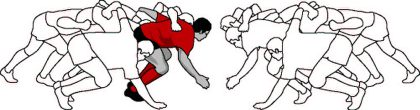
\includegraphics[scale=.45]{img/scrum-rugby.png}
\end{center}
}

\end{frame}

\begin{frame}{{\em Framework} \insertlecture}\small
\begin{columns}
\begin{column}{.5\textwidth}
  \begin{block}<1->{Papeis}\scriptsize
    \begin{itemize}
    \item Proprietário do produto ({\em Product Owner});
    \item Mestre Scrum (Scrum {\em Master});
    \item Equipe ({\em Team}).
    \end{itemize}
  \end{block}
  \pause
  \begin{block}<2->{Cerimônia}
    \begin{itemize}
    \item Planejamento
    \item Revisão
    \item Retrospectiva
    \item Reunião diária
    \end{itemize}
  \end{block}  
\end{column}
\begin{column}{.5\textwidth}
  \begin{block}<3->{Artefatos}
    \begin{itemize}
    \item {\em Backlog} do produto
    \item {\em Backlog} do {\em sprint}
    \item {\em Burndown charts}
    \end{itemize}
  \end{block}
\end{column}
\end{columns}
\end{frame}

\begin{frame}[fragile]{\insertlecture}{Elementos}
  \begin{center}
    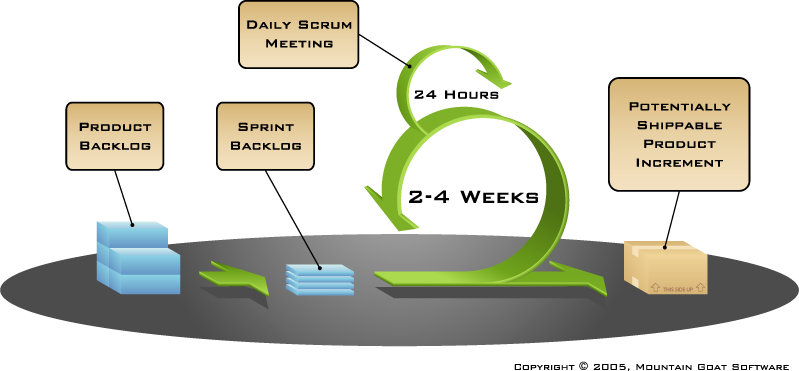
\includegraphics[scale=.4]{img/scrum.png}
  \end{center}
\end{frame}

\begin{frame}{Proprietário do Produto}{{\em Product Owner}}
  \begin{itemize}[<+-| alert@+>]\setbeamercovered{transparent}
  \item Define as funcionalidades do produto;
  \item Define as datas de lançamento;
  \item Prioriza as funcionalidades de acordo com o valor de mercado;
  \item Ajusta funcionalidades e prioridades;
  \item Aceita ou rejeita o resultado dos trabalhos.
  \end{itemize}
\end{frame}

\begin{frame}{Mestre Scrum}{Scrum {\em Master}}
  \begin{itemize}[<+-| alert@+>]\setbeamercovered{transparent}
  \item Representa a gerência do projeto;
  \item Responsável pela aplicação dos valores e práticas do Scrum;
  \item Remove obstáculos;
  \item Garante plena funcionalidade e produtividade da equipe;
  \item Garante a colaboração entre as diversas funções;
  \item Serve como escudo para interferências externas.
  \end{itemize}
\end{frame}

\begin{frame}{Equipe}{Team}
  \begin{itemize}[<+-| alert@+>]\setbeamercovered{transparent}
  \item Entre 5 e 9 pessoas;
  \item Multifuncional: programadores, analistas, testadores, desenvolvedores de 
    interface gráfica, dentre outros;
  \item Tempo integral;
  \item Auto-organizável;
  \item Trocas só nas mudanças de {\em sprints}.
  \end{itemize}
\end{frame}

\begin{frame}{Reunião de Planejamento do Sprint}{\em Sprint Planning Meeting}
\small
\begin{itemize}[<+-| alert@+>]\setbeamercovered{transparent}
\item No início do ciclo de sprint (a cada 7-30 dias), uma Reunião de
  Planejamento de {\em Sprint} é realizado.  
\item O objetivo é selecionar o trabalho que precisa ser feito;
\item Preparar o {\em Sprint Backlog} que detalha o tempo que
  levará para fazer esse trabalho, com toda a equipe.  
\item   Identificar e comunicar o quanto o trabalho é susceptível de ser feito durante a
  sprint atual.  
\item Dividida em duas partes: 
  \begin{enumerate}
    \item  Proprietário do produto: diálogo para priorizar o Product
  Backlog.  
\item Cronograma de um  plano para o {\em Sprint}, resultando na {\em Sprint Backlog}.  
\end{enumerate}
\end{itemize}

\pause\bigskip No final de um ciclo de {\em sprint}, são realizadas duas
reuniões: para \alert{revisão} ({\em Sprint Review}) e
\alert{retrospectiva} ({\em Sprint Retrospective}).
\end{frame}

\begin{frame}{Exemplo de planejamento de {\em sprint}}
  \begin{block}{{\em sprint backlog}}
  \begin{center}
    \begin{tabular}[ht]{|l|c|}\hline
      \bf\hfil Tarefa & \bf Tempo (h) \\\hline
      modelagem & 8 \\\hline
      interface gráfica & 24 \\\hline
      manual do usuário & 16 \\\hline
      testes de unidade & 16 \\\hline
      módulo de armazenamento & 32 \\\hline
    \end{tabular}
  \end{center}
\end{block}
\end{frame}

\begin{frame}{Reunião Diária}\small
  \begin{itemize}[<+-| alert@+>]\setbeamercovered{transparent}
  \item A reunião começa precisamente no horário marcado;
  \item Todos são bem-vindos, mas poucos falam;
  \item A reunião tem duração máxima de 15 minutos;
  \item A reunião deve acontecer no mesmo local e hora todos os dias;
  \item Durante a reunião, cada membro da equipe responde à 3 perguntas:
    \begin{enumerate}
    \item O que você tem feito desde ontem em direção à meta?
    \item O que você está planejando hoje para seguir em direção à meta?
    \item Você tem algum problema impedindo-o de atingir a meta?
    \end{enumerate}
  \end{itemize}

  \pause\bigskip
  É papel do Mestre Scrum facilitar a resolução destes impedimentos.
\end{frame}

\begin{frame}{{\em Backlog} do Produto}{{\em Product Backlog}}
  \begin{itemize}[<+-| alert@+>]\setbeamercovered{transparent}
  \item Uma lista de \alert{requisitos} desejados no projeto;
  \item Idealmente, na forma em que cada item tenha seu peso de acordo com a vontade do cliente ou usuários;
  \item Priorizado pelo proprietário do produto;
  \item Repriorizado no início de cada {\em sprint}.
  \end{itemize}
\end{frame}

\begin{frame}{Exemplo de {\em Backlog} do produto}
  \begin{center}
    \begin{tabular}[ht]{|l|c|}\hline
      \bf\hfil Requisito & \bf\hfil Prioridades \\\hline
      Permitir que o usuário faça uma reserva & 3 \\\hline 
      Permitir a troca de datas da reserva & 3 \\\hline 
      Permitir que o usuário cancele a reserva & 5 \\\hline 
      Permitir que o empregado gere relatório & 8 \\\hline
      Melhorar manipulação de erros & 10 \\\hline
    \end{tabular}
  \end{center}
\end{frame}

\begin{frame}{{\em Backlog} do \em{Sprint}}{{\em Sprint Backlog}}
\begin{itemize}[<+-| alert@+>]\setbeamercovered{transparent}
\item Cada indivíduo escolhe o trabalho que fará;
\item Trabalhos nunca são atribuídos;
\item Atualização diária da estimativa do trabalho restante;
\item Qualquer membro da equipe pode adicionar, apagar ou mudar tarefas;
\item O trabalho aparece a partir do {\em Sprint};
\item Se uma tarefa não é clara, defina-a como um item com uma quantidade maior de tempo e subdivida-a depois;
\item Atualize as coisas a serem feitas na medida em que se tornam mais conhecidas.
\end{itemize}
\end{frame}

\begin{frame}{Exemplo {\em Backlog} do \em{Sprint}}{{\em Sprint Backlog}}

\begin{center}
\begin{tabular}{|l|c|c|c|c|c|}\hline
\bf\hfil Tarefa& \bf seg &\bf  ter & \bf qua &\bf  qui &\bf  sex \\\hline
Codificar interface de usuário & 8 & 4 & 4 & & \\\hline
Codificar regra de negócio  & 16 & 12 & 10 & 4& \\\hline
Testar  & 8 & 16 & 16 & 11 & 8 \\\hline
Escrever {\em help online}  & 12 &  &  & & \\\hline
Escrever a classe X  & 8 & 8 & 8 & 8& 8\\\hline
Adicionar log de erros  &  &  & 8 & 4 & \\\hline
\end{tabular}
\end{center}
\end{frame}

\frame{
  \begin{center}
    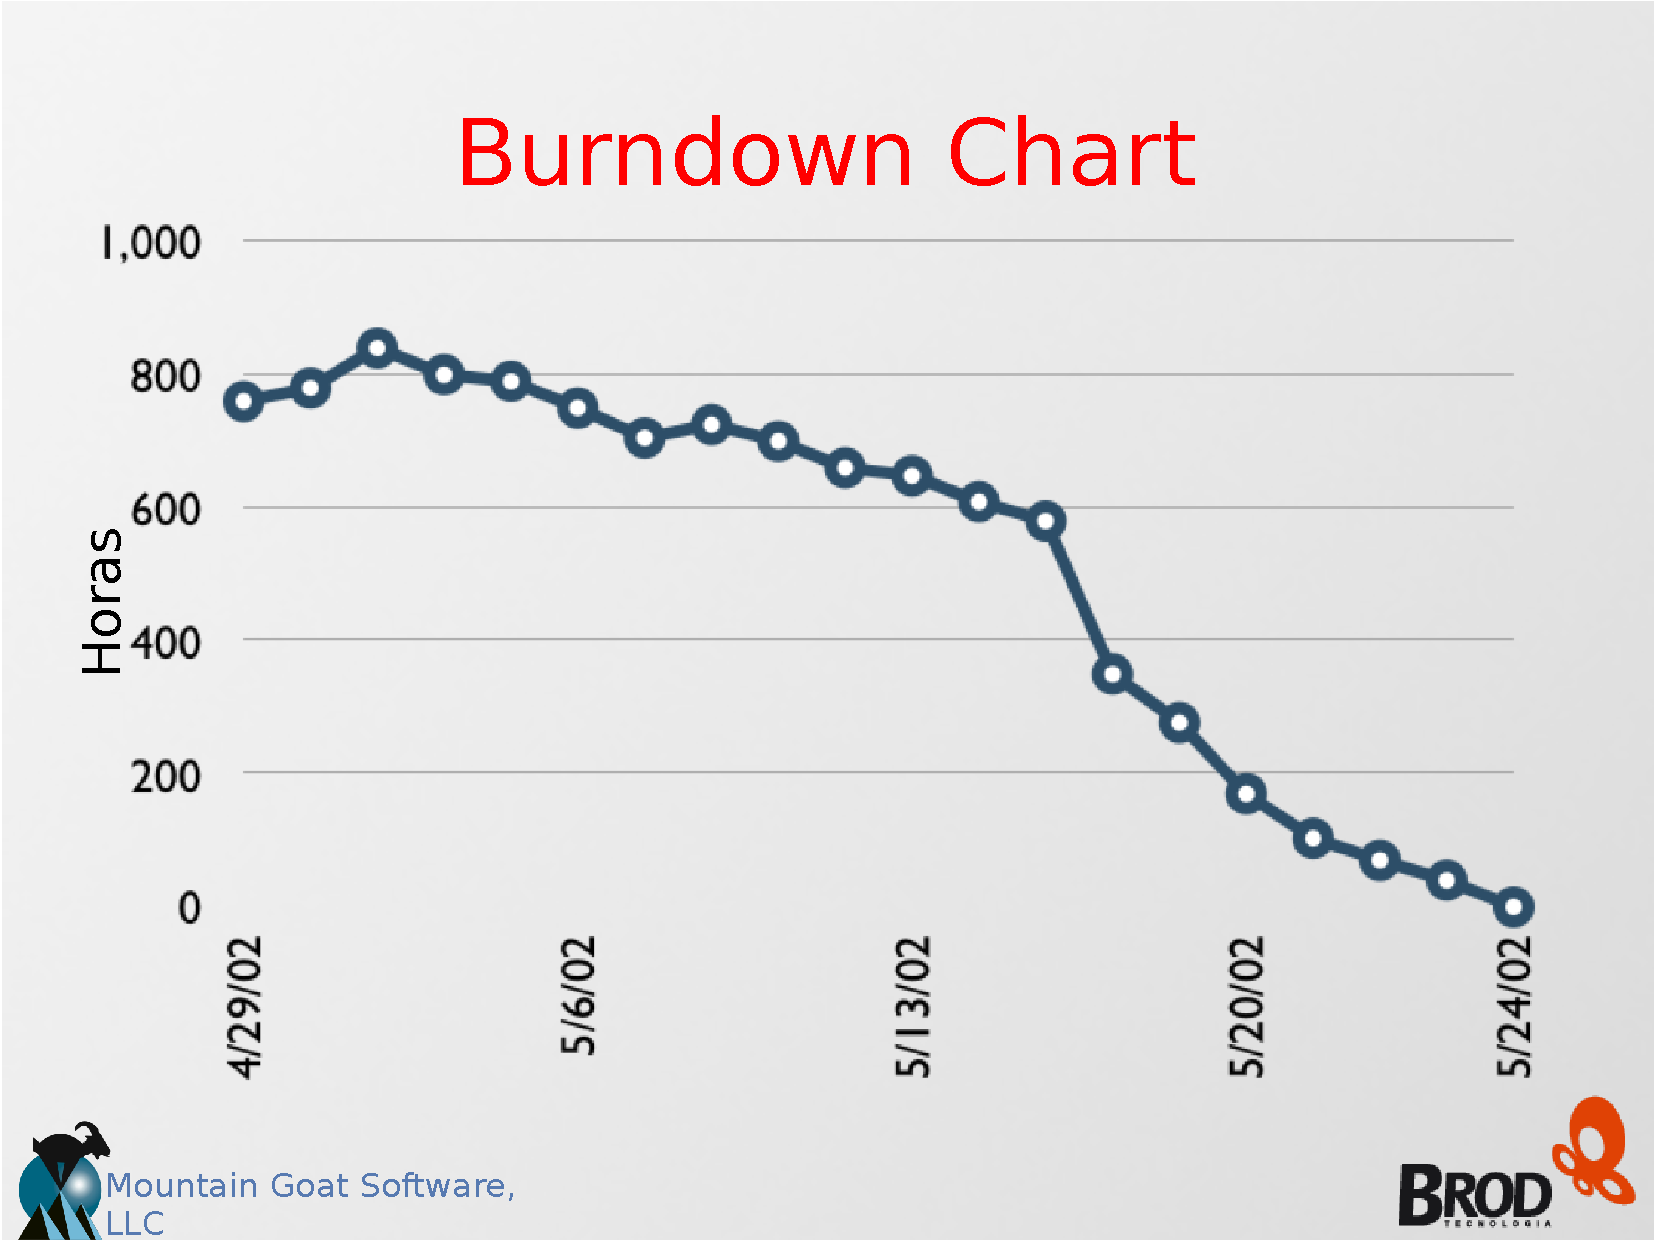
\includegraphics[scale=.35]{img/burndown-chart.pdf}
  \end{center}
}

%%%%%%%%%%%%%%%%% EXTREME PROGRAMMING %%%%%%%%%%%%%%%%
\lecture{\em Extreme Programing (XP)}{xp}
\lecturetitle{\insertlecture}{\course}
\frame{\maketitle}

\begin{frame}{\insertlecture}{Introdução}

  \alert{\insertlecture{}} é uma metodologia de ágil de
  desenvolvimento de software criada por Kent Beck, que foi lider de
  um projeto de um sistema para a Chrisler em 1996, e começou a
  refinar os princípios.
  
  \only<1>{
    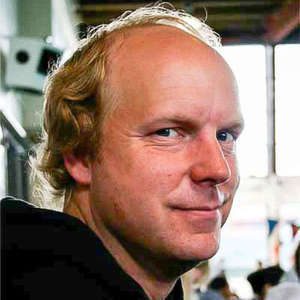
\includegraphics{img/kent-beck.png}
  }
  \pause
  
  \bigskip
  O livro {\em ``Extreme Programming Explained''} escrito por Beck foi 
  lançado em 1999.
\end{frame}

\begin{frame}{Princípios}{\insertlecture}
  
  \begin{description}[<+-| alert@+>]\setbeamercovered{transparent}
  \item[Comunicação:] o programador deve comunicar-se constantemente,
    com o cliente para extrair os requisitos, e com os outros
    programadores, dando ênfase ao trabalho em equipe.
  \item[Simplicidade:] o modelo deve ser o mais simples possível.
  \item[{\em Feedback:}] o software deve ser testado desde o início para 
    que haja {\em feedback} para possíveis alterações.
  \item[Coragem:] o programador pode realizar alterações no código até 
    mesmo na fase final de desenvolvimento.
  \end{description}

\end{frame}

\begin{frame}{Componentes}{\insertlecture}
  \small
  \begin{description}[<+-| alert@+>]\setbeamercovered{transparent}
  \item[Histórias do usuário:] ({\em User stories}) são histórias
    escritas pelo cliente e que descrevem os requisitos do sistema.
  \item[Plano de lançamento:] ({\em release planning}) é o plano a 
    ser seguido durante o desenvolvimento do sistema. Este plano é 
    elaborado pelos programadores e cliente e deve ser baseado em 4 
    valores:
    \begin{enumerate}
    \item \alert{Escopo}: quanto precisa ser feito.
    \item \alert{Recursos}:quantas pessoas estão disponíveis.
    \item \alert{Tempo}: quando o lançamento precisa ser feito.
    \item \alert{Qualidade}: o quão bom será o sistema e os testes.
    \end{enumerate}
  \item[Iteração:] Antes de cada iteração um reunião é feita para 
    escolher a história do usuário a ser implementada.
  \item[Desenvolvimento:] durante o desenvolvimento são feitas
    reuniões todas as manhãs para solucionar problemas e manter o
    foco.
  \end{description}

\end{frame}

\begin{frame}{Componentes}{\insertlecture}
  \begin{description}
  \item[Cartões CRC:] (CRC--Classe, Responsabilidade e Colaboração)
    contem informações sobre o modelo do sistema de forma
    simplificada, permitindo a colaboração entre os programadores.

  \end{description}
  \footnotesize
    Cartão CRC \\ 
  \begin{tabular}[h]{|lll|}\hline
    \multicolumn{3}{|l|}{{\bf Nome da Classe:} SensorMovimento (subclasse de Sensor)}\\\hline
    \multicolumn{3}{|l|}{Tipo de classe: dispositivo, concorrente}\\ \hline
    \multicolumn{3}{|l|}{Características de classe: tangível}\\ \hline
    \multicolumn{2}{|l|}{\bf Responsabilidades} & \multicolumn{1}{|l|}{\bf Colaboração}\\
    \multicolumn{2}{|l|}{} & \multicolumn{1}{|l|}{}\\                                         
    \multicolumn{2}{|l|}{{\tt registraEvento(eventoSensor)}: registra evento do sensor} & \multicolumn{1}{|l|}{EventoSensor}\\
    \multicolumn{2}{|l|}{} & \multicolumn{1}{|l|}{}\\                                         
    \multicolumn{2}{|l|}{{\tt estaAtivo()}: relata se o sensor está ativo} & \multicolumn{1}{|c|}{---}\\
    \multicolumn{2}{|l|}{} & \multicolumn{1}{|l|}{}\\                                         
   \multicolumn{2}{|l|}{{\tt reset()}: reconfigura o sensor.} & \multicolumn{1}{|c|}{---}\\\hline
  \end{tabular}
\end{frame}

\begin{frame}{Componentes}{\insertlecture}
  \begin{description}[<+-| alert@+>]\setbeamercovered{transparent}
  \item[Metáfora do sistema:] forma padronizada de se referir aos elementos do 
    sistema (classes, objetos e métodos), para que possam ser reutilizados.
  \item[Propriedade coletiva do código:] o código é de propriedade da equipe, 
    sendo que qualquer membro pode alterá-lo.
  \item[Teste de unidade:] os testes são escritos pelos programadores 
    antes de começarem a implementação, para dar um melhor entendimento 
    dos requisitos.
  \item[Teste de aceitação:] o cliente especifica cenários para testar 
    as funcionalidades durante o preparo das histórias.
  \item[Velocidade:] a velocidade do projeto está ligada à 
    quantidade de histórias implementada em cada iteração.
  \end{description}
\end{frame}

\begin{frame}{Componentes}{\insertlecture}
  \begin{description}[<+-| alert@+>]\setbeamercovered{transparent}
  \item[Pequenos lançamentos:] são feitos pequenos lançamentos a partir 
    das iterações para capturar o {\em feedback} do cliente.
  \item[Modelagem simplificada:] a modelagem é mantida a mais simples 
    possível para facilitar o entendimento e alterações.
  \item[Programação em pares:] cada tarefa é realizada por um par de programadores 
    trabalhando colaborativamente.
  \item[{\em Refactoring:}] é a remoção de código duplicado ou alteração de um código 
    que não está simples.
  \item[Integração contínua:] a codificação é feita pela junção de pequenas tarefas 
    feitas e testadas separadamente. A cada iteração, todo o código deve ser integrado 
    e os testes de unidade realizados com sucesso.
  \item[40 horas:] Cada programados trabalha somente 40 horas por semana.
  \end{description}
\end{frame}

\begin{frame}{Referência}

  \begin{itemize}
  \item {\em Extreme Programming Concepts (Software Engineering Series)}. Jessica Keyes.
  \end{itemize}
  
\end{frame}

\lecture{Kanban}{kanban}
\lecturetitle{\insertlecture}{\course}
\frame{\maketitle}

\begin{frame}{\insertlecture}{Introdução}
  
  \begin{itemize}[<+-| alert@+>]\setbeamercovered{transparent}
  \item No final da década de 1940, a Toyota começou a modernizar seus
    processos de Engenharia baseando-se no mesmo modelo que os
    supermercados usavam para repor produtos na prateleira.
  \item O objetivo era ter em estoque somente o necessário para a
    produção em um determinado período de tempo, técnica chamada {\em
      Just In Time} (JIT).
  \item Quando um material acabava no piso da fábrica, um cartão ({\em
      kanban}\footnote{{\em Kanban} é uma palavra japonesa que
      significa sinal visual.}) era passado para o estoque informando
    a quantidade exata de material que deveria ser reposta.
  \end{itemize}
  
\end{frame}

\begin{frame}{\insertlecture}{Software}

  \begin{itemize}[<+-| alert@+>]\setbeamercovered{transparent}
  \item As equipes de desenvolvimento agil de software usam os
    princípios de JIT para alinhar a quantidade de trabalho em 
    andamento com a capacidade da equipe.
  \item O fluxo de trabalho é controlado e monitorado através do uso
    de cartões, dando flexibilidade de planejamento, clareza no foco e
    maior transparência.
  \end{itemize}

\end{frame}

\begin{frame}{Cartões Kanban}
  
  \begin{itemize}[<+-| alert@+>]\setbeamercovered{transparent}
  \item Todo o trabalho das equipes kanban gira em torno de um 
    quadro kanban, usado para visualizar o fluxo de trabalho 
    na equipe.
  \item O fluxo de trabalho é identificado visualmente e padronizado, 
    com os bloqueios e dependências identificados e resolvidos.
  \item Um fluxo de trabalho básico pode ser dividido em 3 colunas:
    {\bf A Fazer}, {\bf Fazendo} e {\bf Feito}.
  \end{itemize}

  \only<4>{
  \begin{center}
    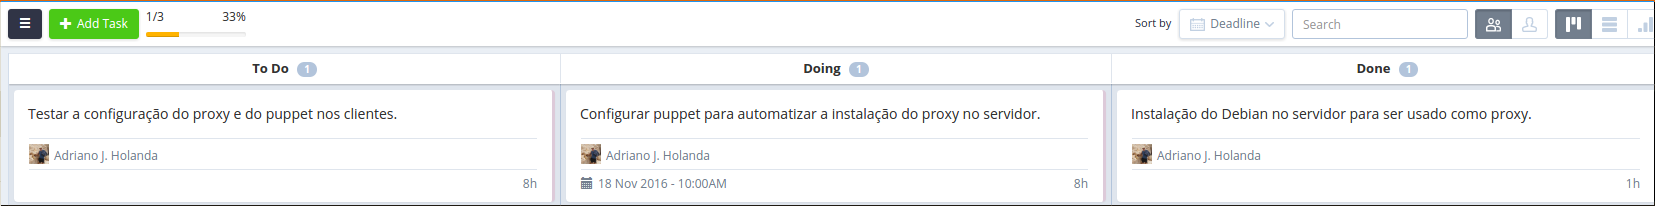
\includegraphics[scale=.2]{img/kanban-board.png}
  \end{center}
}

\end{frame}

\begin{frame}{Cartões Kanban}

  \begin{center}
    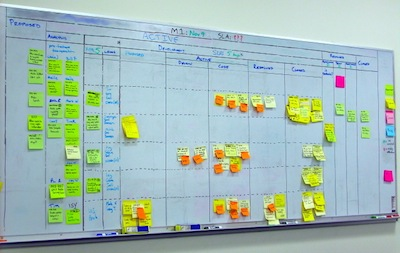
\includegraphics[scale=.5]{img/kanban-projeto.png}\\
    \bigskip
    Exemplo de um quadro Kanban.
  \end{center}

\end{frame}

\begin{frame}{\insertlecture}{Benefícios}
  \begin{description}[<+-| alert@+>]\setbeamercovered{transparent}
  \item[Flexibilidade no planejamento:] há uma liberdade a respeito das
    escolhas de quais tarefas a serem executadas.
  \item[Ciclo de tempo reduzido:] A métrica principal no Kanban é o ciclo 
    de tempo, que é o tempo que uma unidade de trabalho leva para 
    percorrer os estados definidos. Portanto, o foco deve estar 
    na otimização deste ciclo.
  \item[Métrica visual:] A métrica pode ser facilmente entendida e 
    acompanhada.
  \item[Entrega contínua:] associada à integração contínua, novas
    funcionalidades ou reparos de {\it bugs} são integrados
    rapidamente ao produto ou serviço.
  \end{description}
\end{frame}

\begin{frame}{Scrum $\times$ Kanban}
  
  O Scrum e o Kanban compartilham alguns conceitos, porém, apresentam
  algumas diferenças de abordagens:

\begin{center}\footnotesize
  \begin{tabular}[h]{|l|l|l|}\hline
    & \hfil\bf\color{blue} Scrum & \hfil\bf\color{red} Kanban \\\hline\hline
    Cadência & \color{blue} Sprints de tamanho fixo & \color{red} Fluxo contínuo \\\hline
    Metodologia de &\color{blue} Ao final de cada sprint aprovado&\color{red} Entrega contínua ou \\
    lançamento     &\color{blue} pelo proprietário do produto  &\color{red} a critério da equipe\\\hline
    Papéis &\color{blue} Proprietário do produto, &\color{red} Sem papéis fixos, \\
         &\color{blue} scrum {\it master} e equipe  &\color{red} podendo haver um gerente. \\\hline
    Mudanças & \color{blue} Somente entre os sprints &\color{red} A qualquer tempo \\\hline
  \end{tabular}
\end{center}

\end{frame}

\begin{frame}{Questionário\footnote{Sommerville, 2011}}\small
  {\bf Um não sugere Ágil; um sim sugere Planejar-Documentar.}\\
  \begin{enumerate}
  \item A especificação é requerida?
  \item Os clientes não estão disponíveis?
  \item O sistema a ser construído é grande?
  \item O sistema a ser construído é complexo (por exemplo, tempo real)?
  \item O produto terá um tempo de vida longo?
  \item Você está usando ferramentas de software de baixa qualidade?
  \item A equipe do projeto está geograficamente distribuída?
  \item A equipe é parte de uma cultura orientada à documentação?
  \item A equipe tem poucas habilidades de programação?
  \item O sistemas a ser construído está sujeito à regulação?
  \end{enumerate}

\end{frame}

\begin{frame}{Referências}
  \begin{itemize}
  \item \href{https://www.atlassian.com/agile/kanban}{``Kanban: How
      the kanban methodology applies to software development''.  Dan
      Radigan. Atlassian Inc.}
  \item
    \href{https://feituverava.bv3.digitalpages.com.br/users/publications/9788579361081}{I. Sommerville. Engenharia
      de Software. Editora Pearson, 9a edição, 2011.}
  \end{itemize}
\end{frame}
